\chapter{Introduction}
\label{chap:introduction}
%=====================================================

% A introdução geral do documento pode ser apresentada através das seguintes seções: Desafio, Motivação, Proposta, Contribuição e Organização do documento (especificando o que será tratado em cada um dos capítulos). O Capítulo 1 não contém subseções\footnote{Ver o Capítulo \ref{cap-exemplos} para comentários e exemplos de subseções.}.


%=====================================================

As computers grow in power and shrink in size, more aspects of everyday life can be enhanced by adding processing units to common devices.
While many of these applications focus on conveniences, such as home automation \cite{mccole2016} (the collection of connected and smart devices is dubbed the Internet of Things or IoT \cite{morgan2014}), the integration of computers with other objects and devices can also be important to save time and save lives \cite{rti2014}.
One way of achieving this is by adding computers and wireless transmitters to vehicles — such as cars, buses, and trains — so they can share data which may increase traffic efficiency or reduce the chance of accidents \cite{saini2015close}.

In 2013, an estimated 1.25 million people lost their lives due to traffic accidents globally \cite{whotraffic}.
While this number has greatly reduced over the past decades \cite{johnson2010traffic} thanks to better safety features (seat belts, air bags, ABS, etc.) and stronger laws (drunk driving, motorcycle helmets, speed limits, etc.), it may still rise as a major cause of death in the years to come \cite{whofactsheet}, so further actions are necessary.
Furthermore, as the car population increases, congestions consume ever more time of the daily commuter, peaking at over 100 hours per year for the residents of Los Angeles, CA \cite{inrixtraffic}.

Smart vehicles and vehicular networks are ways that technology can aid both of the aforementioned problems.
Through the use of sensors and wireless communications, these vehicles are able to avoid accidents by alerting distracted drivers \cite{lee2004collision}, or by knowing in advance another vehicle's position and speed \cite{hafner2011automated}.
By communicating, they can also collaborate to offer driving and route suggestions, therefore reducing the possibility of traffic jams \cite{knorr2012reducing}.
%These features are possible with the development of a vehicular ad-hoc network (VANET), in which vehicles can quickly share data amongst themselves without the need of a server or an Internet connection.

When dealing with safety or traffic-efficiency applications, it is crucial that network communications occur with low latency (approximately 100 milliseconds \cite{camp2005vehicle}).
Current cellular technology, such as LTE, could be used to connect vehicles to the Internet, but the delay added by the transmission would make safety applications unfeasible or unreliable \cite{mangel2010comparison}.
Cellular connections also have other problems: the connection would require an active subscription with a carrier; the connection depends on available infrastructure; the wireless frequency would be shared with phones and other mobile devices, increasing the possibility of interference and congestion; server-side issues could impact the vehicles' communications.

For these reasons, ad-hoc solutions are preferred over centralized ones.
An ad-hoc network is one that has no reliance on pre-existing infrastructure (such as routers or access points) \cite{wu2004ad}.
Instead, each node is able to communicate directly with others and a routing protocol allows for messages to be forwarded until they reach their destinations.
Every time a node wants to send a message and the recipient is not a direct neighbor, it must choose which nearby node is the most likely one to get the message to its destination.
Routing techniques can use either the network's topology or geographical coordinates \cite{saini2015close} to choose which node should be the next hop.

These issues — the additional safety and efficiency as well as the low-latency communications — can be tackled through the use of a vehicular ad-hoc network (VANET), in which vehicles share data amongst themselves without relying on external devices, an Internet connection or server availability.
Neighboring vehicles can share their position and velocity data at high frequencies, allowing, for example, for autonomous vehicles to plan a platooning approach to traffic \cite{amoozadeh2015platoon}.
In the case of a collision or other event, nearby nodes can broadcast alerts, which other nodes pick up and forward \cite{li2007routing}.
That way, an alert can travel long distances in little time, allowing approaching vehicles to safely slow down or pick alternative routes.

\begin{figure}[h]
    \centering
    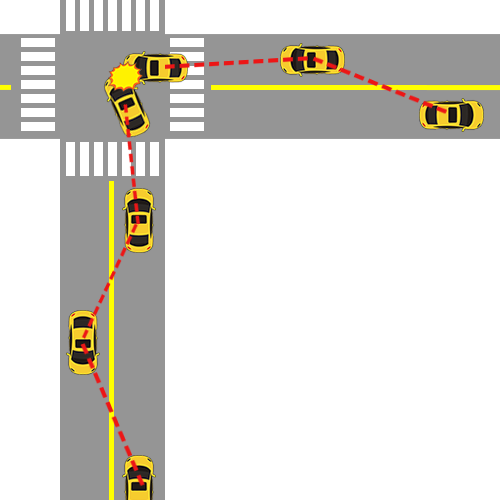
\includegraphics[width=0.5\textwidth]{images/collision.png}
    \caption{Propagation of a collision alert in a VANET}
    \label{fig:collision}
\end{figure}

As is the case with most new technologies, VANETs are expected to be a notable target of attacks for a diversity of reasons \cite{isaac2010security}.
A local malicious user might alter the data his or her vehicle broadcasts in order to manipulate traffic conditions, while remote attackers could invade vehicles' computers and obtain partial control of the network  \cite{garip2015congestion}.
These attacks can vary from time-consuming annoyances to life-threatening, so it is important that real-world implementations of vehicular networks are prepared to handle them.

%However, as is the case for many types of networks, VANETs must be reliable in order to be functional.

%In the case of ad-hoc networks, the nodes themselves must be reliable, since data can only propagate safely through benign cooperation.

%In ad-hoc networks, the secure propagation of data depends on the reliability of each node, since messages often travel 

%While in a conventional technological network (such as the Internet), the 
In ad-hoc networks, one way to mitigate a number of attacks is through each node using data collected from previous experiences to filter out incoming messages that seem to be malicious, incorrect, or irrelevant.
A node's degree of confidence that some data is correct and useful is called \textit{trust}.
%The ability of nodes to verify one another and judge messages based on past experiences is called \textit{trust}.
% The product of a series of past experiences with one other node is called trust.
For instance, in the example of a single malicious user broadcasting false data, nodes receiving these messages can use their own sensors to verify whether or not the data was correct, and update the \textit{trust value} of the sender vehicle.
In case the trust value of a sender is too low, a receiver node can choose to ignore the data contained in a message, as it concluded that the sender is not trustworthy.
Trust allows for better cooperation of nodes in a network, since incorrect messages might be detected and discarded.

Furthermore, once nodes form their own opinions about others, they can propagate pre-existing trust values when necessary.
For example, if two nodes are not direct neighbors and do not have any pre-existing trust information about each other, they can ask intermediary nodes for their opinions on the other node \cite{wang2009trust}.
The management of trust values (i.e. how one node acquires and updates trust values) and the use of these values to derive further information (such as designating nodes as malicious or not) is called \textit{trust management} \cite{ma2011survey}. 
%The combination of one node's trust of another with the opinions of other nearby nodes form what is called \textit{trust management}.
The effective use of trust management allows for the detection of malicious, misbehaving or faulty nodes in the network, and for such information to be shared amongst the benign participants. 
Throughout this document, trust and trust management may be used interchangeably.

%There is an important distinction between \textit{trust} and \textit{trust management}.
%The former relates to the actual trust relationship between a pair of nodes, while the latter concerns the management of previously generated trust data, such as previous tests or information received from neighboring nodes, and how this data can be used to make decisions.
%While this work addresses trust management rather than trust itself, both terms will be used when referring to trust management for the sake of brevity.
%Without trust management\footnote{} features, a vehicle cannot judge whether or not received messages are benign or malicious in order to make an informed decision and, therefore, incorrect data might be presented to the driver.

While the detection of incorrect nodes and/or messages is an important aspect of security and safety in vehicular networks, it does not address all of the problems.
Trust solutions are not viable without a solid identity verification scheme, for instance, since nodes would not be able to form trust opinions without being sure of the others' identities (these schemes often use a Public Key Infrastructure \cite{wasef2010complementing}).
They also do not address issues such as driver and passenger privacy when using the facilities of a VANET.
Furthermore, cryptography must be used in order to guarantee that the secrecy of messages is not violated.
Therefore, trust and trust management must be viewed as an important aspect of vehicular ad-hoc networks, but not as a definitive solutions to all of the related concerns.

In order to study the implications of trust in vehicular networks, it is interesting to first take a closer look at trust in other kinds of networks.
VANETs are a subset of technological networks, therefore it is useful to consider how the Internet or other ad-hoc networks handle trust.
Furthermore, VANETs contain several features often found in social networks, which can be directly tied to how nodes form and develop trust relationships with each other.

%While this work emphasizes on the characteristics of VANETs, they are only a subset of the much broader field of complex networks.
%The study of complex networks dates back decades, including analysis of biological or social networks \cite{wang2003complex} \cite{newmannetworks}.
%Trust issues are present in many of these types of networks, although each one requires a specific approach that addresses the peculiarities involved.

%Often, when people hear the term ``network'', they think only of technological examples, such as computer networks.
%Such networks are only a subset of a much larger field of study: that of complex networks.
%The study of complex networks dates back decades, including analysis of biological or social networks \cite{wang2003complex} \cite{newmannetworks}.
%Technological networks, and VANETs by extension, are only a subset of that much larger field of study.
%
%Trust issues and their solutions are an important aspect of the study of complex networks, and of social or technological networks in particular.
%Each different type of network requires a specific approach to trust, according to the features that distinguish it from others.
%It is interesting to review the solutions proposed for social networks and technological networks in general, and then narrow down on how dynamic networks, and VANETs in particular, are handled.
%Despite the differences, there are some concepts that overlap across most types of networks.

This work proposes a method for identifying malicious nodes in a vehicular network, although it may also be viable for other dynamic and decentralized networks.
The solution is based on a previously existing algorithm \cite{vernize2015malicious}, which was limited to centralized networks.
In order to adapt the algorithm to a dynamic and decentralized environment, it is necessary to locate network features that allow for trust relationships to be developed amongst the network members over time, since there is no centralizing agent to store and process the whole network's trust values.
These features are found by tracing analogies to social networks, i.e. identifying how and why two nodes (in the case of VANETs, vehicles) would meet more than once and at a somewhat predictable interval.

% Seems like there's a paragraph missing to explain why we mention social and technological networks at all.

%Further explain VANETs

%VANETs can be complex networks

%why mention social networks

\section{Document organization}
The remainder of this document is organized as follows. \Cref{chap:complexnetworks} explains the broad study of complex networks and the importance of trust in technological and social networks.
Then, \autoref{chap:vanets} goes into details regarding VANETs and the importance of trust solutions in the field, presenting previous studies made on the subject.
Finally, \autoref{chap:proposal} shows the fundamentals of this proposed work, including the similarities found between VANETs and social networks, a realistic movement model that may be used for simulations, the previously existing study on malicious node identification for complex networks, and the important aspects that must be adapted to the dynamic vehicular environment.